%% Mathematical Geosciences (Springer Nature sn-jnl, Math & Physical Sciences
%% Author-Year Reference Style -- author-year citation confirmed in the
%% journal's official submission guidelines).
%% Publishable engine only -- transport (warped) kriging is patent-pending and
%% excluded from this manuscript.
\documentclass[pdflatex,sn-mathphys-ay]{sn-jnl}

\usepackage{graphicx}
\usepackage{booktabs}
\usepackage{amsmath}
\usepackage{siunitx}
\usepackage{natbib}
\graphicspath{{../../figures/}}

\raggedbottom

\begin{document}

\title[Unifying native, Python and WebAssembly geostatistics]{geostat-rs: unifying native, Python and WebAssembly geostatistics from a single const-generic Rust core}

\author*[1]{\fnm{Francisco} \sur{Parra-O.}}\email{}

\affil*[1]{\orgaddress{\country{Chile}}}

\abstract{Geostatistical methods are implemented independently across at
least six actively maintained tools --- gstat (R), GSLIB (Fortran), GSTools,
SciKit-GStat and PyKrige (Python), and GeoStats.jl (Julia) --- each tied to a
single language runtime and deployment target, with no core shared between
server, desktop and in-browser execution. We present geostat-rs, architected
to close this fragmentation: a single Rust core, generic over spatial
dimension (2-D and 3-D from one const-generic code path, with no
per-dimension code duplication), compiles unchanged to three deployment
targets --- a dependency-light native binary, a Python extension module
(PyO3, zero-copy NumPy arrays) and WebAssembly for in-browser execution with
no server --- and uses a deterministic random-number generator so stochastic
simulation is bit-identical across all three. The engine covers experimental
and theoretical variography; the kriging family
(simple/ordinary/universal/external-drift, co-kriging, indicator and block
kriging); inverse-distance and $k$-nearest-neighbour baselines; regression
kriging; and conditional sequential Gaussian and indicator simulation. We
show this architecture costs no numerical fidelity: every deterministic
method is cross-checked against gstat on the Meuse and Walker Lake
benchmarks at machine precision, and simulation is validated
distributionally. Accuracy is assessed by VEcv (variance explained by
cross-validation), and regression kriging accepts an externally supplied
trend --- letting a machine-learning model provide the mean while geostat-rs
kriges the residuals. We demonstrate the engine on a Chilean national
mine-tailings geochemistry dataset, predicting rare-earth grades from
host-mineral proxies. The engine reads and writes OGC GeoPackage without
GDAL, for native interchange with GIS tools.}

\keywords{geostatistics, kriging, Rust, cross-validation, regression kriging, GeoPackage}

\maketitle

\section{Introduction}\label{sec:intro}

Spatially continuous fields --- ore grades, element concentrations, soil and
environmental variables --- are increasingly required across ecology, agronomy,
geochemistry, mining and environmental science, yet are rarely measured
exhaustively: they must be predicted from sparse point samples
\citep{li2021,goovaerts1997}. Geostatistics supplies the established machinery
for this --- variography to characterise spatial dependence, kriging to predict
with quantified uncertainty, and stochastic simulation to represent it --- and a
growing body of work couples it with machine learning for the trend component
\citep{hengl2018}. A practitioner therefore needs a single tool that spans this
whole workflow, validates against an accepted reference, and deploys without a
heavy runtime.

The consequence is that the same methods are implemented independently at
least six times over. gstat \citep{pebesma2004} is comprehensive and the
de-facto reference, but is bound to the R runtime, single-threaded in its
hot paths, and offers no single-binary or in-browser deployment; GSLIB
\citep{deutsch1998} is fast, canonical Fortran but arcane and without modern
packaging, bindings or a Python/WebAssembly interface. The Python
geostatistics ecosystem --- GSTools \citep{mueller2022}, SciKit-GStat
\citep{maelicke2022} and PyKrige \citep{pykrige} --- is convenient and
scriptable but pure-Python in performance and tied to the Python runtime;
GeoStats.jl \citep{hoffimann2018} closes much of the performance gap with a
compiled, high-performance core in Julia, but offers neither single-binary
deployment nor Python or WebAssembly bindings. No shared numerical core spans
server, desktop and in-browser execution: each of these six tools re-derives
and re-validates the same variogram models and kriging systems independently,
in a different language, for a different single deployment target.

We present geostat-rs to close that fragmentation architecturally, rather than
add a seventh independent implementation. Its design goals are: (i) one
numerical core, generic over spatial dimension via Rust's const generics, so
2-D and 3-D share a single code path with no per-dimension duplication;
(ii) that same core compiled unchanged to three deployment targets --- a
dependency-light native binary, a Python extension module, and WebAssembly for
client-side execution with no server; (iii) a deterministic random-number
generator so stochastic simulation is bit-identical across all three targets;
(iv) numerical parity with gstat, to show the architecture costs no fidelity
relative to the field's reference implementation; and (v) a
predictive-accuracy-first evaluation methodology with a bridge to machine
learning, following \citet{li2021}. Our contributions are this const-generic,
multi-target architecture itself; its validation against gstat at machine
precision as evidence that unifying the core does not trade away numerical
fidelity; predictive-accuracy tooling (VEcv-based comparison and tuning); an
ML+geostatistics hybrid through regression kriging; GeoPackage input/output;
and a real rare-earth application. Sect.~\ref{sec:design} describes the
engine's design and implementation; Sect.~\ref{sec:methods} summarizes the
methods it covers; Sect.~\ref{sec:validation} and Sect.~\ref{sec:performance}
report validation against gstat and performance; Sect.~\ref{sec:accuracy}
compares methods by predictive accuracy; Sect.~\ref{sec:application}
demonstrates a real application; and Sect.~\ref{sec:discussion} discusses
limitations and future work.

\section{Design and implementation}\label{sec:design}

geostat-rs is written in Rust (edition 2024) as a Cargo workspace:
geostat-core (the library, with no I/O and only light dependencies),
geostat-cli (a command-line tool), geostat-python (a PyO3
module, abi3 $\geq$ 3.9) and geostat-wasm (WebAssembly with a browser
demo). The core is generic over the spatial dimension through a const-generic
PointSet<const D>, so variography, kriging, cross-validation and
simulation run unchanged in 2-D and 3-D. Moving neighbourhoods use a $k$-d tree;
sequential simulation uses an incremental bucket grid. A deterministic
random-number generator (xoshiro256++) makes simulation reproducible:
the same seed yields identical realizations on any platform. Native parallelism
(rayon) is behind a feature flag that is disabled for the wasm32 target. The
Python module reproduces the CLI bit-for-bit, and the WebAssembly build runs
the same engine in the browser with no server (Fig.~\ref{fig:wasm}).

\begin{figure}[t]
\centering
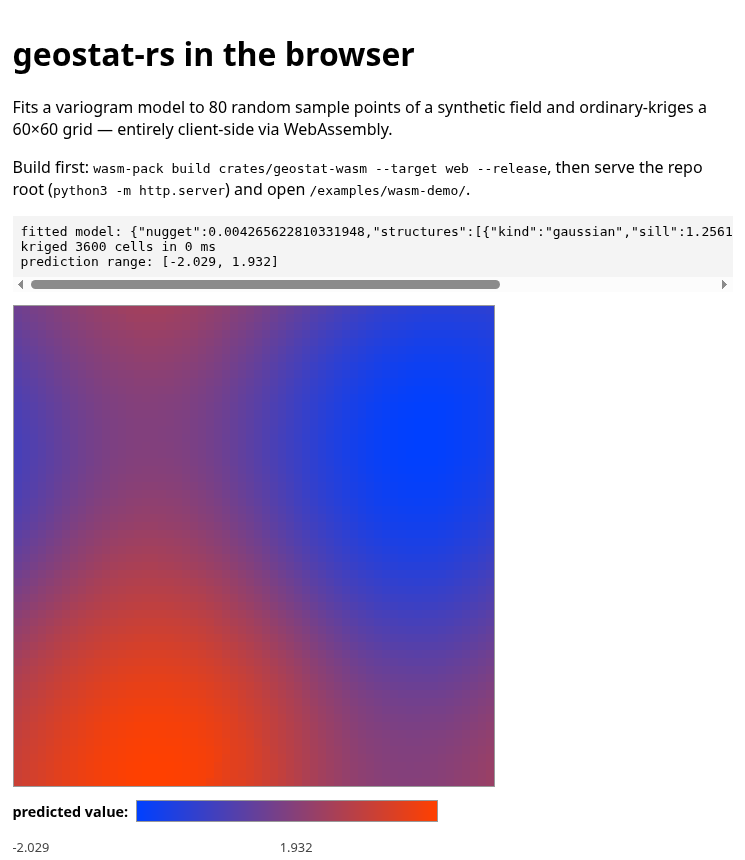
\includegraphics[width=0.7\linewidth]{fig_wasm.png}
\caption{The WebAssembly build running entirely client-side in a browser: it
fits a variogram and ordinary-kriges a $60\times60$ grid of a synthetic field,
rendering the prediction surface on a canvas with a colour-scale legend.}
\label{fig:wasm}
\end{figure}

\section{Methods}\label{sec:methods}

\textbf{Variography.} Experimental variograms (omnidirectional, directional with
azimuth and a 3-D dip cone), a 2-D variogram map for diagnosing anisotropy, and
cross-variograms; theoretical models (spherical,
exponential, Gaussian, Mat\'ern $\nu=3/2,5/2$), nested with a nugget and with
geometric anisotropy; weighted-least-squares fitting with gstat's default
$N_j/h_j^2$ weights via Nelder--Mead, with automatic best-family selection and
optional joint fitting of geometric anisotropy (major-axis azimuth and
minor/major ratio) across directional variograms. On Meuse log-zinc
(Fig.~\ref{fig:anis}) the fit recovers the textbook NE--SW continuity of the
river floodplain (major azimuth $\approx 36^\circ$, minor/major ratio
$\approx0.24$), consistent with the elongation of the variogram map.

\begin{figure}[t]
\centering
\includegraphics[width=\linewidth]{fig_anisotropy.pdf}
\caption{Anisotropy of Meuse log-zinc. (a) The 2-D variogram map; the dashed
line marks the fitted major axis. (b) Directional experimental variograms along
the fitted major and minor axes (point size proportional to pair count) with the
jointly fitted anisotropic model. The major axis (NE--SW, $\approx 36^\circ$)
has the longer range; the minor axis reaches the sill within ${\sim}900$\,m.}
\label{fig:anis}
\end{figure}

\textbf{Kriging.} Simple, ordinary, universal (polynomial drift) and
external-drift kriging, following the classical formulations of
\citet{journel1978} and \citet{chiles2012}; ordinary co-kriging (collocated and
heterotopic) under a linear model of coregionalization \citep{chiles2012};
block kriging and block co-kriging; indicator kriging (local ccdf, E-type
estimate, conditional variance); and lognormal kriging.

\textbf{Mathematical interpolators.} Inverse-distance weighting and
$k$-nearest-neighbour averaging ($k=1$ is nearest-neighbour / Voronoi) as
assumption-light baselines for fair comparison \citep{li2021}.

\textbf{Regression kriging.} A trend is fitted in a separate first step ---
either the built-in ordinary-least-squares trend or any external model --- and
the residuals are kriged and added back. Decoupling the trend lets it come from
any regressor, including machine learning \citep{hengl2018,li2021}.

\textbf{Simulation.} Conditional sequential Gaussian simulation (normal-score
transform) and sequential indicator simulation with order-relation corrections,
both with the deterministic generator.

\textbf{Predictive-accuracy tooling.} Following \citet{li2016}, leave-one-out
cross-validation reports VEcv ($=100\,[1-\sum(y-\hat y)^2/\sum(y-\bar y)^2]$, a
scale- and variance-independent cross-validated $R^2$) and the Legates--McCabe
$E_1$, alongside scale-free relative measures. A harness ranks methods by VEcv
on the same data, and hyperparameters (IDW power, $k$-NN $k$, kriging
neighbourhood size) are tuned by maximizing VEcv rather than by a model fit.

\textbf{Input/output.} CSV; OGC GeoPackage point layers (read and write) and
single-band 2D-gridded-coverage raster (read and write, integer datatype),
implemented in pure Rust via bundled SQLite and a PNG codec, i.e.\ without a
GDAL dependency; a read raster can be sampled at point locations to attach a
covariate (e.g.\ a DEM) for external-drift or regression kriging.

\section{Validation against gstat}\label{sec:validation}

Every deterministic method is cross-checked against gstat on the Meuse and
Walker Lake benchmarks. Table~\ref{tab:parity} lists headline parities; the full
tables are in the repository. Conventions are aligned with gstat where they
matter: the semivariance estimator, right-closed lag bins, $N_j/h_j^2$ fit
weights, azimuth measured clockwise from north and nugget-free within-block
covariance. Figure~\ref{fig:parity} shows geostat-rs against gstat on the Meuse
grid for ordinary kriging and IDW: predictions lie on the identity line to
machine precision. Simulation is validated distributionally --- a
1000-realization sequential Gaussian ensemble reproduces the theoretical
simple-kriging mean and standard-deviation fields and the pooled quantiles,
while running about $7\times$ faster than gstat.

\begin{table}[t]
\centering
\caption{Maximum difference between geostat-rs and gstat (Meuse / Walker Lake).}
\label{tab:parity}
\begin{tabular}{@{}lll@{}}
\toprule
Method & Check & Max difference \\
\midrule
Experimental variogram & $\gamma$ (relative), 15 lags & \num{1.6e-15} \\
Ordinary kriging & meuse.grid, 3103 cells & \num{1.5e-12} \\
LOO cross-validation & 155 points & \num{9.7e-13} \\
KED / anisotropy / co-kriging & predictions & $\leq$\,\num{1.5e-12} \\
Block / 3-D / heterotopic co-kriging & predictions & $\leq$\,\num{4e-14} \\
Indicator kriging (in range) & $F(\text{cutoff})$ & \num{7.4e-10} \\
Lognormal (simple) kriging & vs gstat SK + analytic & \num{1.2e-9} \\
Inverse-distance weighting & power 2, global & \num{1.9e-14} \\
\botrule
\end{tabular}
\end{table}

\begin{figure}[t]
\centering
\includegraphics[width=\linewidth]{fig_parity.pdf}
\caption{geostat-rs versus gstat predictions on the Meuse grid for ordinary
kriging and inverse-distance weighting; points lie on the identity line (dashed)
to machine precision.}
\label{fig:parity}
\end{figure}

\section{Performance}\label{sec:performance}

Table~\ref{tab:bench} times ordinary kriging on regular grids of increasing
size and leave-one-out cross-validation, conditioning on the 155 Meuse points
with a 32-point moving neighbourhood and the same fitted model. Only the
operation is timed (data preloaded, best of three runs); geostat-rs is timed
through its Python binding (a thin wrapper over the Rust compute) against
gstat~2.1.4. Single-threaded, geostat-rs is already faster than gstat at grid
kriging ($1.2$--$2\times$); with its parallel moving-neighbourhood predictor on
16 cores it is $6$--$12\times$ faster. Leave-one-out cross-validation is far
faster still, as gstat's krige.cv carries per-fold R-level overhead
that the parallel Rust implementation avoids. For a global neighbourhood the
kriging-system matrix is identical for every target, so geostat-rs factorizes it
once (LU) and only back-substitutes per target, an order-of-magnitude saving on
large grids.

\begin{table}[t]
\centering
\caption{Wall-clock time (ms, best of 3) for ordinary kriging and
leave-one-out cross-validation. Hardware: 12th-gen Intel Core i7-1270P
(16 logical cores); gstat 2.1.4 single-threaded.}
\label{tab:bench}
\begin{tabular}{@{}lrrrr@{}}
\toprule
Task & gstat & \shortstack[r]{geostat-rs\\(1 core)} &
\shortstack[r]{geostat-rs\\(16 cores)} & speedup \\
\midrule
OK grid, 2\,500 cells   & 184  & 89   & 15  & $12\times$ \\
OK grid, 10\,000 cells  & 570  & 472  & 60  & $10\times$ \\
OK grid, 40\,000 cells  & 2173 & 1595 & 341 & $6\times$ \\
LOO cross-validation (155 pts) & 1368 & 8.9 & 5.2 & $263\times$ \\
\botrule
\end{tabular}
\end{table}

\section{Predictive accuracy, comparison and tuning}\label{sec:accuracy}

On Meuse log-zinc, leave-one-out VEcv ranks ordinary kriging
($\approx 71$, 95\% bootstrap CI $[60, 79]$) above IDW ($\approx 55$, CI
$[44, 63]$), $k$-NN ($\approx 54$, CI $[41, 65]$) and nearest-neighbour
($\approx 38$, CI $[15, 57]$) (Fig.~\ref{fig:compare}; CIs from 2000
resamples of the leave-one-out pairs). Ordinary kriging's advantage over IDW
and $k$-NN is robust to this resampling, but IDW and $k$-NN's own CIs overlap
almost entirely --- their point estimates are close enough that this dataset
cannot distinguish between them. No method dominates universally, so the
comparison is by measured predictive accuracy rather than assumption.
Hyperparameters are tuned the same way: Figure~\ref{fig:idwtune} shows IDW power
selected by VEcv, with an optimum near power~3.5 on this dataset.

\begin{figure}[t]
\centering
\includegraphics[width=0.85\linewidth]{fig_compare.pdf}
\caption{Leave-one-out VEcv by method on Meuse log-zinc, with 95\% bootstrap
confidence intervals.}
\label{fig:compare}
\end{figure}

\begin{figure}[t]
\centering
\includegraphics[width=0.85\linewidth]{fig_idw_tune.pdf}
\caption{IDW power tuned by predictive accuracy (leave-one-out VEcv) on Meuse
log-zinc.}
\label{fig:idwtune}
\end{figure}

\section{Application: rare-earth grade prediction in Chilean mine tailings}\label{sec:application}

We predict rare-earth grades in 1118 samples from 331 mine-tailings
deposits in the Coquimbo region, drawn from the public geochemical registry of
tailings deposits in Chile \citep{sernageomin2023}, from non-rare-earth
host-mineral proxies (P$_2$O$_5$, Th for phosphates/monazite; TiO$_2$,
Fe$_2$O$_3$, Zr for Ti--Fe oxides and zircon), deliberately excluding
neighbouring rare-earth elements, which are co-measured and would constitute
leakage. Samples of one deposit lie close together: under a random hold-out the
median distance from a test location to its nearest training location is
31~m, so every method can borrow within-deposit autocorrelation. We therefore
hold out whole deposits. Each of 20 splits sends about a quarter of the
locations to the test set, deposit by deposit, which raises that median
distance to 156~m; Table~\ref{tab:ree} and Fig.~\ref{fig:ree} report the mean
and standard deviation of hold-out VEcv over the splits.

Held out by deposit, ordinary kriging has no skill for Ce, Nd or Dy (mean VEcv
between $-1.7$ and $-0.8$\%) and little for Y (18.1\%): the spatial correlation
it exploits operates within deposits, not between them. The host-mineral
proxies carry the signal --- the random forest explains 53.7\%, 63.2\%,
36.6\% and 53.3\% of the variance of Ce, Nd, Dy and Y --- while La is predicted
by no method (every mean is negative; the engine does not manufacture signal).
The random-forest-trend plus residual-kriging hybrid outperforms regression
kriging with a linear trend wherever signal exists (by 4.1 to 9.5 points), but
it ties the random forest itself for Ce, Nd and Dy (paired differences of
$-0.4$ to $+0.4$ points, standard deviation about 1) and gains only for Y
($+1.8 \pm 0.9$ points). Random location splits, by contrast (crosses in
Fig.~\ref{fig:ree}), inflate the VEcv of both kriging variants by 9 to 13
points for Ce, Nd, Dy and Y and credit the hybrid with a 1.2 to 4.2 point gain
over the random forest: residual kriging adds value only where same-deposit
samples are near, and a random hold-out mistakes that proximity for
predictive skill. The random-forest trend is supplied by a companion Rust
machine-learning engine and the residual kriging by geostat-rs, giving an
RFOK-style hybrid \citep{li2021} with no R or scikit-learn dependency.
These proxy--target relationships are specific to the Coquimbo tailings'
mineralogy and this single regional dataset; we report them as a demonstration
of the engine's regression-kriging bridge to machine learning; they are not a
general claim about rare-earth prediction from host-mineral proxies in other
geological settings.

\begin{table}[t]
\centering
\caption{Hold-out VEcv (\%) by rare-earth element and method (Coquimbo
tailings; host-mineral proxies), held out by deposit: mean (standard
deviation) over 20 splits. Skew of the grade is shown for context. Computed
with geostat-rs 0.8.0 and smelt 0.8.1 (\texttt{figures/make\_figure\_data.py}).}
\label{tab:ree}
\begin{tabular}{@{}lrrrrr@{}}
\toprule
Element & skew & OK & RK (OLS) & RF & RF+res.\ krige \\
\midrule
La & 10.3 & $-26.2$ (69) & $-12.4$ (64) & $-17.0$ (30) & $-16.6$ (40) \\
Ce & 5.9 & $-1.7$ (19) & 47.8 (23) & 53.7 (18) & 54.1 (17) \\
Nd & 6.2 & $-1.5$ (16) & 53.3 (20) & 63.2 (13) & 62.8 (14) \\
Dy & 3.0 & $-0.8$ (7) & 32.7 (15) & 36.6 (13) & 36.8 (14) \\
Y  & 0.5 & 18.1 (7) & 48.5 (6) & 53.3 (6) & 55.1 (6) \\
\botrule
\end{tabular}
\end{table}

\begin{figure}[t]
\centering
\includegraphics[width=\linewidth]{fig_multielement.pdf}
\caption{Rare-earth grade prediction by element and method. Bars: hold-out
VEcv held out by deposit, mean $\pm$ one standard deviation over 20 splits
(axis truncated at $-45$\%; La's intervals extend further). Crosses: mean
over random location splits, which leak within-deposit autocorrelation.
Ordinary kriging loses most of its skill once deposits are held out; the
residual-kriging hybrid then ties the random forest except for Y.}
\label{fig:ree}
\end{figure}

\section{Discussion and limitations}\label{sec:discussion}

geostat-rs shows that a single Rust core can deliver the classical
geostatistical workflow --- variography, the kriging family and stochastic
simulation --- at numerical parity with gstat while adding cross-platform
reproducibility, native parallelism, and Python and in-browser deployment from
one code base. Pairing that core with a predictive-accuracy-first evaluation
layer (VEcv-based comparison and tuning) and bring-your-own-trend regression
kriging connects classical geostatistics to the machine-learning workflow
without leaving the engine or adding an R or scikit-learn dependency.

Several limitations bound the present scope. Kriging systems are solved by dense
LU factorization: this is robust for the moving-neighbourhood regime that
dominates practice, and for a global neighbourhood the single-factorization
reuse keeps large grids tractable, but it does not target the very large dense
or sparse systems for which approximate or covariance-tapering solvers would be
required. Computation is CPU-only and single-machine --- there is no GPU path
and no out-of-core or distributed mode --- so problem size is bounded by memory.
GeoPackage support reads and writes vector points and integer raster coverages,
but the float (TIFF-tile) coverage datatype and additional formats remain to be
added.
Validation and benchmarking here target the classical datasets (Meuse, Walker
Lake) and a single regional application; a broader empirical study across data
types and scales is left for future work, and the predictive-accuracy
comparison is deliberately confined to the methods in the engine rather than
surveying the wider machine-learning literature. The Meuse method comparison
(Sect.~\ref{sec:accuracy}) reports bootstrap confidence intervals on VEcv; the
rare-earth application (Sect.~\ref{sec:application}) reports the mean and
standard deviation over 20 deposit-grouped splits; with a few hundred
deposits those deviations stay large (13 to 23 points for Ce and Nd), so its
element-by-element VEcv values should be read as a demonstration of the
regression-kriging bridge rather than as precise estimates.

Future directions include GPU and out-of-core execution for larger grids,
additional input/output formats and full GeoPackage raster support for tighter
GIS interchange, and broader application studies. The deterministic,
dependency-light design is intended to make geostat-rs usable both as a
standalone tool and as an embeddable component of larger Rust geocomputing
pipelines, with results that remain reproducible across the platforms on which
it runs.

\section{Software availability and reproducibility}\label{sec:availability}

geostat-rs is released as open-source software under a dual MIT/Apache-2.0
license, with crates for the core, CLI, Python and WebAssembly bindings, at
\url{https://github.com/franciscoparrao/geostat-rs}. All validations are
reproduced by the R reference scripts and Python comparison scripts in the
repository, and all figures by the provided data-generation and plotting
scripts. Results are deterministic and platform-independent. The Meuse and
Walker Lake benchmark datasets are distributed with gstat; the
rare-earth application uses the public geochemical registry of tailings
deposits in Chile \citep{sernageomin2023}, openly available from the national
geology and mining service.

\backmatter

\bmhead{Acknowledgements}
%% TODO

\section*{Declarations}

\bmhead{Funding}
%% TODO

\bmhead{Conflict of interest}
The author declares no conflict of interest.

\bmhead{Data availability}
The Meuse and Walker Lake benchmark datasets are distributed with the R
package gstat. The rare-earth tailings dataset is openly available from
SERNAGEOMIN's public tailings registry \citep{sernageomin2023}.

\bmhead{Code availability}
geostat-rs is open source (MIT/Apache-2.0) at
\url{https://github.com/franciscoparrao/geostat-rs}.

\bibliography{refs}

\end{document}
